\documentclass{article}
\usepackage[margin=0.75in]{geometry}
\usepackage[utf8]{inputenc}

% Get better typography
\usepackage[protrusion=true,expansion=true]{microtype}  
% For algorithms
\usepackage[boxruled,linesnumbered,vlined,inoutnumbered]{algorithm2e}
\SetKwInOut{Parameter}{Parameters}
% For basic math, align, fonts, etc.
\usepackage{amsmath}
\usepackage{amsthm}
\usepackage{amssymb}
\usepackage{mathtools}
\usepackage{mathrsfs}
\usepackage{rotating}
\usepackage{gensymb} % For \degree
\usepackage{lscape}
% For \thead to make line breaks in tables
\usepackage{array}
\usepackage{makecell}
\renewcommand\theadalign{bc}
\renewcommand\theadfont{\bfseries}
\renewcommand\theadgape{\Gape[4pt]}
\renewcommand\cellgape{\Gape[4pt]}
\usepackage{courier} % For \texttt{foo} to put foo in Courier (for code / variables)
\usepackage{lipsum} % For dummy text
% For images
\usepackage{graphicx}
\usepackage{subcaption}
\usepackage[space]{grffile} % For spaces in image names
% For bibliography
\usepackage[round]{natbib}
% For color
\usepackage{xcolor}
\definecolor{light-grey}{rgb}{0.9,0.9,0.9}
\definecolor{dark-red}{rgb}{0.4,0.15,0.15}
\definecolor{dark-blue}{rgb}{0,0,0.7}
\usepackage{environ}
% Only show sections in table of contents and rename
\setcounter{tocdepth}{2}
\renewcommand{\contentsname}{Table of Contents}
% For links (e.g., clicking a reference takes you to the phy)
\usepackage{hyperref}
\hypersetup{
    colorlinks, linkcolor={dark-blue},
    citecolor={dark-blue}, urlcolor={dark-blue}
}

\newcommand{\TODO}[1]{\textcolor{blue}{\textbf{{#1}}}}
\newcommand{\POINTS}[1]{\textcolor{purple}{\textbf{{#1}}}}


\begin{document}


%-----------------
%   Homework 1
%-----------------
\newpage
\begin{center}
    \begin{Large}
    CMPSCI 687 Homework 1 - Fall 2022 
    \end{Large}
    \\
    Due \TODO{September 30, 2022}, 11:55pm Eastern Time
\end{center}
\addcontentsline{toc}{subsection}{\textbf{Homework 1}}

\textcolor{blue}{\textbf{Note: we have added comments, below, to clarify some of the problems/questions in this homework. All parts of this document that were changed with respect to the original one are shown in blue.}}

\section{Instructions}

This homework assignment consists of a written portion and a programming portion. While you may discuss problems with your peers (e.g., to discuss high-level approaches), you must answer the questions on your own. In your submission, do explicitly list all students with whom you discussed this assignment. Submissions must be typed (handwritten and scanned submissions will not be accepted). You must use \LaTeX. The assignment should be submitted on Gradescope as PDF with marked answers via the Gradescope interface. The source code should be submitted via the Gradescope programming assignment as a .zip file. Include with your source code instructions for how to run your code. You \textbf{must} use Python 3 for your homework code. You may not use any reinforcement learning or machine learning specific libraries in your code, e.g., TensorFlow, PyTorch, or scikit-learn. You \textit{may} use libraries like numpy and matplotlib, though. The automated system will not accept assignments after 11:55pm on September 30. The tex file for this homework can be found \href{https://people.cs.umass.edu/~bsilva/courses/CMPSCI_687/Fall2022/HWs/HW1.zip}{here}. 

\section{Hints and Probability Review}
\label{sec:hints}
    \begin{itemize}
        \item \textbf{Write Probabilities of Events:} In some of the probability hints below that are not specific to RL, we use expressions like $\Pr(a|b)$, where $a$ and $b$ are events.  Remember that in the RL notation used for this class, the values of $\Pr(s_0)$, $\Pr(a_0)$, $\Pr(A_0)$, or $\Pr(A_0 | S_0)$ are all undefined, since those are simply states, actions, or random variables (not events).  Instead, we \underline{\textbf{\textit{must}}} write about the probabilities of events.  For example: $\Pr(A_0 = a_0)$ or $\Pr(A_0 = a_0 | S_0 = s_0)$.
        %
        \item \textbf{Bayes' Theorem:} $\Pr(a|b) = \frac{\Pr(b|a) \Pr(a)}{\Pr(b)}$. This is useful for dealing with conditional probabilities $\Pr(a|b)$ if the event $a$ occurs \textit{before} event $b$.  For example, it is often difficult to work with an expression like $\Pr(S_0 = s_0 | A_0 = a_0)$, because the agent \textit{first} observes the current state, $S_0$, and only afterwards selects an action, $A_0$; in this case, it is much easier to deal with the 3 terms in $\frac{\Pr(A_0 = a_0 | S_0 = s_0) \Pr(S_0 = s_0)}{\Pr(A_0 = a_0)}$.
        %
        \item \textbf{The law of total probability:} For event $a$, and a set of events $\mathcal{B}$,
        $$\Pr(a) = \sum_{b \in \mathcal B} \Pr(b) \Pr(a|b)$$ See the example below for several useful applications of this property.
        \item \textbf{``Extra'' given terms:} Remember that when applying laws of probability, any ``extra'' given terms stay in the result.  For example, applying the law of total probability: $$\Pr(a|c,d) = \sum_{b \in \mathcal B} \Pr(b|c,d) \Pr(a|c,d,b)$$
        %
        \item \textbf{Conditional Probabilities - Useful property \#1:} If you need to move terms from the ``right-hand side'' of a conditional probability to the ``left-hand side'', you can use the following identity:  \\
        $\Pr(a|b,c) = \frac{\Pr(a,b|c)}{\Pr(b|c)}$ 
        %
        \item \textbf{Conditional Probabilities - Useful property \#2:} If you need to move terms from the ``left-hand side'' of a conditional probability to the ``right-hand side'', you can use the following identity:  \\
        $\Pr(a,b|c) = \Pr(a|b,c)P(b|c)$
        %
        \item \textbf{Expected Values:} The expected value of a random variable $X$ with possible outcomes in $\mathcal{X}$ is $$\mathbb{E}[X] = \sum_{x \in \mathcal{X}} x \Pr(X=x)$$
        %
        \item \textbf{Conditional Expected Values:} The expected value of a random variable $X$ with possible outcomes in $\mathcal{X}$, conditioned on an event $A=a$, is $$\mathbb{E}[X\,|\,A=a] = \sum_{x \in \mathcal{X}} x \Pr(X=x \,|\, A=a )$$
        %

        \item \textbf{Example problem:} The probability that the state at time $t = 1$ is $s \in \mathcal S$. 
        \begin{align}
        \Pr(S_1 = s) =& \sum_{s_0 \in \mathcal S} \Pr(S_0 = s_0) \Pr(S_1 = s | S_0 = s_0) \\
        %
        =& \sum_{s_0\in \mathcal S} d_0(s_0) \Pr(S_1 = s | S_0 = s_0)\\
        %
        =& \sum_{s_0\in \mathcal S} d_0(s_0) \sum_{a_0\in \mathcal A} \Pr(A_0 = a_0 | S_0 = s_0)\\
        &\times \Pr(S_1 = s | S_0 = s_0, A_0 = a_0)\\
        %
        =& \sum_{s_0\in \mathcal S} d_0(s_0) \sum_{a_0\in \mathcal A} \pi(s_0, a_0) \, p(s_0, a_0, s).
        \end{align}
    \end{itemize}
    %

\vspace{0.5cm}
\noindent\rule{\textwidth}{1pt}

\section*{Part One: Written (55 Points Total)}
\begin{enumerate}
    \item \textit{\textbf{(Your grade will be a zero on this assignment if this question is not answered correctly)} Read the class syllabus carefully, including the academic honesty policy. To affirm that you have read the syllabus, type your name as the answer to this problem. }
    %
    % YOUR RESPONSE HERE
    %
    \item (\POINTS{18 Points}) Given an MDP $M=(\mathcal S, \mathcal A, p, R, d_0, \gamma)$ and a fixed policy, $\pi$, the probability that the action at time $t=0$ is $a \in \mathcal A$ is:
    \begin{equation}
        \Pr(A_0=a)=\sum_{s \in \mathcal S} d_0(s) \pi(s,a).
    \end{equation}
    Write similar expressions (using only $\mathcal S,\mathcal A,p,R,d_0,\gamma$, and $\pi$) for the following problems.\\
    
    \textbf{Important:}
    
    \begin{itemize}
    
    \item \emph{Assume, below, that the reward function will be in the form $R: \mathcal{S} \times \mathcal{A} \rightarrow \mathbb{R}$. That is, the reward at time $t$ depends only on the state at time $t$ and action at time $t$.}
    
    \item \emph{All solutions below \underline{need} to be derived from ``first principles'': you should repeatedly apply definitions and properties of probability distributions such as the ones discussed in Section \ref{sec:hints}, as well as the Markov Property (when appropriate), and then replace the relevant quantities with their corresponding definitions in RL (e.g., you can substitute $\Pr(A_0=a|S_0=s)$ with $\pi(s,a)$).} 
    
        \item \textit{Remember that the Markov Property allows you to ignore history information, prior to time $t$, if you know $S_t$ (that is, if the probability term is conditioned on $S_t$). It \underline{does not} allow you to ignore variables associated with time $t$ or any future times ($t+1$, $t+2$, etc). For instance:
        \\
        $$\Pr(S_1=s_1 | A_1=a_1, S_0=s_0) \neq \Pr(S_1=s_1 | S_0=s_0) $$
        \\
        and
        $$\Pr(S_2=s_2 | S_4=s_4, S_1=s_1) \neq \Pr(S_2=s_2 | S_1=s_1).$$}

    \item \emph{When writing the final answers to the problems below (2a-2d), please reorganize your terms and summations in ``temporal'' order. For instance, instead of presenting your final answer as
    \\
    $$\sum_{s_1} p(s_1,a_1,s_2) \pi(s_1,a_1) \sum_{a_0} p(s_0,a_0,s_1) \pi(s_0,a_0)$$
    \\
    \textit{rewrite it as follows:}\\
    $$\sum_{a_0} \pi(s_0, a_0) \sum_{s_1} p(s_0,a_0,a_1) \pi(s_1,a_1) p(s_1,a_1,s_2).$$}
    \end{itemize}
    %
    \vspace{0.25cm}
    \textbf{Problems:}

    \begin{itemize} %[label=\Alph*]
        \item \textbf{(Question 2a.~\POINTS{4 Points})} What is the expected reward at time $t=8$ given that the state at time $t=7$ is $s_7$ and the action at time $t=6$ is $a_6$?
        %
        % YOUR RESPONSE HERE
        %
        \item \textbf{(Question 2b.~\POINTS{4 Points})} What is the probability that the state at time $t=64$ is $s_{64}$ given that the state at time $t=62$ is $s_{62}$?
        %
        % YOUR RESPONSE HERE
        %
        \item \textbf{(Question 2c.~\POINTS{4 Points})} What is the probability that the state at time $t=2$ is $s_{2}$?
        %
        % YOUR RESPONSE HERE
        %
        \item \textbf{(Question 2d.~\POINTS{6 Points})} What is the probability that the state at time $t=5$ \textit{was} $s_5$ given that $A_6=a_6$ and $S_4 = s_4$?
        %
        %
        % YOUR RESPONSE HERE
        %
    \end{itemize}
    
    \item (\POINTS{7 Points}) In class we discussed how reward functions can be used to specify what is the ``goal'' (or objective) of the agent. We presented three ways in which the reward function can be specified: some are extremely general, but not necessarily easy to define in practice; and some are less general but can be defined more intuitively in real-world problems:
    \begin{itemize}
        \item The most general formulation of the reward function is given by $d_R$, which specifies an arbitrary distribution over rewards given that the agent is in some state $s$, executes an action $a$, and transitions to some state $s'$.
        \item Alternatively, in some problems the reward function can be defined in a way that it (deterministically) returns a scalar number based on $s$, $a$, and $s'$. That is, $R$ can be defined as a function of the form $R(s,a,s')$.
        \item Finally, an even simpler formulation of reward functions can be constructed that depends only on the state of the agent ($s$) and the action that it executed ($a$). That is, $R$ can be defined as a function of the form $R(s,a)$.
    \end{itemize}
    %
    Which form of the reward function should be used in practice depends on the particular learning problem or application at hand. In certain problems, for instance, rewards may depend on the state to which the agent transitioned ($s'$) after executing an action ($a$); in this case, using $R(s,a,s')$ may be more convenient. Importantly, all of these definition are closely related, in the sense that we can, for example, write $R(s,a)$ in terms of $d_R$, and $R(s,a)$ in terms of $R(s,a,s')$. 
    \begin{itemize}
        \item \textbf{(Question 3a. \POINTS{4 Points})} First, show from ``first principles'', \textit{step by step}, how to derive an equation for $R(s,a)$ in terms of $d_R$. Recall that, by definition, $R(s,a) = \mathbb E[R_t | S_t = s, A_t = a]$.
        %
        % YOUR RESPONSE HERE
        %
        \item \textbf{(Question 3b. \POINTS{3 Points})} Next, show (again, step by step) how to construct an equation for $R(s,a)$ in terms of $R(s,a,s')$.
    \end{itemize}
        %
        % YOUR RESPONSE HERE
        %
    \item (\POINTS{4 Points}) Suppose you wish to identify an optimal \textit{deterministic} policy for a given MDP with 3 actions and $|\mathcal S|$ states. 
    %
    One way to identify the optimal policy is by performing brute force search; that is, by evaluating $J(\pi)$ for \textit{all} possible deterministic policies $\pi$ and returning the best one; i.e., the one with the highest expected return/performance.
    %
    Assume you are given a black-box software that can evaluate \textit{any} policy defined over this MDP in 5 seconds. Assume you have a total time of two hours to identify the optimal policy.
    %
    Under this time constraint, and assuming you will be using brute force search to identify the optimal policy, what is the maximum number of states, $|\mathcal S|$, that the MDP may have? Show, formally and step by step, how you arrived at your solution.
    %
    % YOUR RESPONSE HERE
    %
    \item (\POINTS{4 Points}) In class, we presented one particular MDP with finite state space and continuous actions, and showed that it \textit{did not} have an optimal policy. Consider an MDP with $|\mathcal S| = \infty$ and $|\mathcal A| < \infty$. Assume $\gamma < 1$. \textit{Formally} define an MDP with these properties (i.e., formally specify all elements of the tuple $(\mathcal{S}, \mathcal{A}, p, R, d_0, \gamma$), where you can assume that $R: \mathcal{S} \times \mathcal{A} \rightarrow \mathbb{R}$) for which an optimal policy, $\pi^*$, \textit{does} exist. Describe such an optimal policy in English and present/describe its performance, $J(\pi^*)$.
    %
    % YOUR RESPONSE HERE
    %
    \item (\POINTS{5 Points}) The objective of standard RL algorithms is to find policies that maximize expected return. However, this objective does not take into account the possible \textit{risks} of deploying such policies. Consider, for example, an optimal policy ($\pi_1)$ that, when executed by the agent, results in a return of $+20$ with 50\% probability, and a return of $-12$ with 50\% probability. Consider an alternative optimal policy ($\pi_2$) that, when executed, produces a return of $+4$  deterministically. The expected return of both policies is the same. One could argue, however, that even though both policies have the same average performance, an agent could prefer policy $\pi_2$ since deploying it would never result in a (possibly catastrophic) low performance---in this particular case, a return of $-12$. RL algorithms have been proposed that identify policies that perform well (i.e., policies with high expected return) but whose \textit{return variance} is small. Intuitively, these algorithms identify policies that, when deployed, produce returns that are both high \textit{and} predictable/reliable. Recall that we defined return as the discounted sum of rewards: $\sum_{t=0}^\infty \gamma^t R_t$. Let an MDP exist such that it has two optimal policies. Can the expected value of their returns differ? If not, explain why; if so, give an example. Furthermore, can the variance of their returns differ? \textcolor{blue}{\textbf{If so, give an example by presenting an \textit{infinite horizon} MDP with two optimal policies whose expected returns are equal, but such that the variance of their corresponding returns differs.}}
    %
    % YOUR RESPONSE HERE
    % 
    \item (\POINTS{3 Points}) To fully specify an MDP we have to define $\mathcal S$, $\mathcal A$, $p$, $R$, $d_0$, and $\gamma$. In many real-world applications, however, it may not be possible (or it might be incredibly challenging) to \textit{specify an explicit/analytic} equation for $R$. Give an example of a real-world problem that can be modeled as an MDP but where $R$ is not known \textit{a priori} by the agent (or cannot be easily specified analytically) and explain why that is the case. Also, describe one possible way by which the agent could incrementally learn/estimate $R$ based on its interactions with the environment.
    %
    % YOUR RESPONSE HERE
    %
    \item (\POINTS{3 Points}) Similarly to the question above, describe a real-world problem that can be reasonably modeled as an MDP, but such that its transition function, $p$, is \emph{not} be known \textit{a priori} by the agent or cannot be easily specified analytically. Explain why that is the case and propose one possible way by which the agent could estimate it based on its interactions with the environment. 
    %
    % YOUR RESPONSE HERE
    %
    \item (\POINTS{6 Points}) Consider an MDP $(\mathcal S, \mathcal A, p, R, d_0, \gamma)$, where we know that the rewards produced by $R$ are bounded between $-R_{\mbox{\small{min}}}$ and $R_{\mbox{\small{max}}}$. Assume that someone gives you a policy, $\pi$, whose return is $J(\pi) = \dfrac{R_{\mbox{\small{max}}}}{1 - \gamma}$. What can you say about the suboptimality of this policy? Is there a way of bounding how much worse $J(\pi)$ may be when compared to the expected return of an optimal policy, $J(\pi^*)$? Can an alternative policy, $\pi_{\mbox{\small{new}}}$, be constructed that has higher return than $\pi$? If so, explain intuitively how; if not, \textit{prove} why this cannot be done.
    %
    % YOUR RESPONSE HERE
    %
    \item (\POINTS{5 Points}) Consider the \href{https://en.wikipedia.org/wiki/Dinosaur\_Game}{Dinosaur Game}---a browser game developed by Google and built into the Google Chrome web browser. The player controls a pixelated Tyrannosaurus rex across a side-scrolling landscape, avoiding obstacles to achieve  high scores. For a demo of this game, please see this \href{https://www.youtube.com/watch?v=2apVwq-pX9E}{video}. Assume we wish to model this game as an MDP so that an RL agent can be trained to optimally control the dinosaur. Assume that the state includes information about the current velocity of the dinosaur and its distance to the next obstacle. Assume there are only two actions: Jump or Do\_Nothing. Suppose that $\gamma=1$ and that the MDP is finite-horizon; in particular, the game either terminates after 100,000 steps or if the agent collides with an obstacle (in which case the episode ends). The reward function returns $+1$ after each action that keeps the dinosaur alive, and $0$ otherwise. To make the game more challenging, its developers implemented a rule that changes the speed with which the dinosaur moves: its speed increases automatically after every 100 steps. This means that, e.g., at time $t=23$, the dinosaur might be moving $5$ meters ahead after every action; at time $t=140$, however, the dinosaur might be moving $7.5$ meters ahead after every action. Using the formal definition of stationary and non-stationary MDPs, introduced in class, show formally that this is a non-stationary MDP. Furthermore, describe precisely how you would change the definition of this MDP (i.e., the definition of one or more components of $(\mathcal S, \mathcal A, p, R, d_0, \gamma)$) so that the resulting MDP does model the game as describe above, and so that it is stationary. Use the formal definitions of stationarity and non-stationarity to formally show that this new MDP is, indeed, stationary.
\end{enumerate}

\newpage
%\vspace{1cm}
\section*{Part Two: Programming (45 Points Total)}

Consider the following MDP:
% \\ \\
% \textbf{[[Image omitted]]}
% \\ \\
\begin{figure}[h!!!]
    \centering
    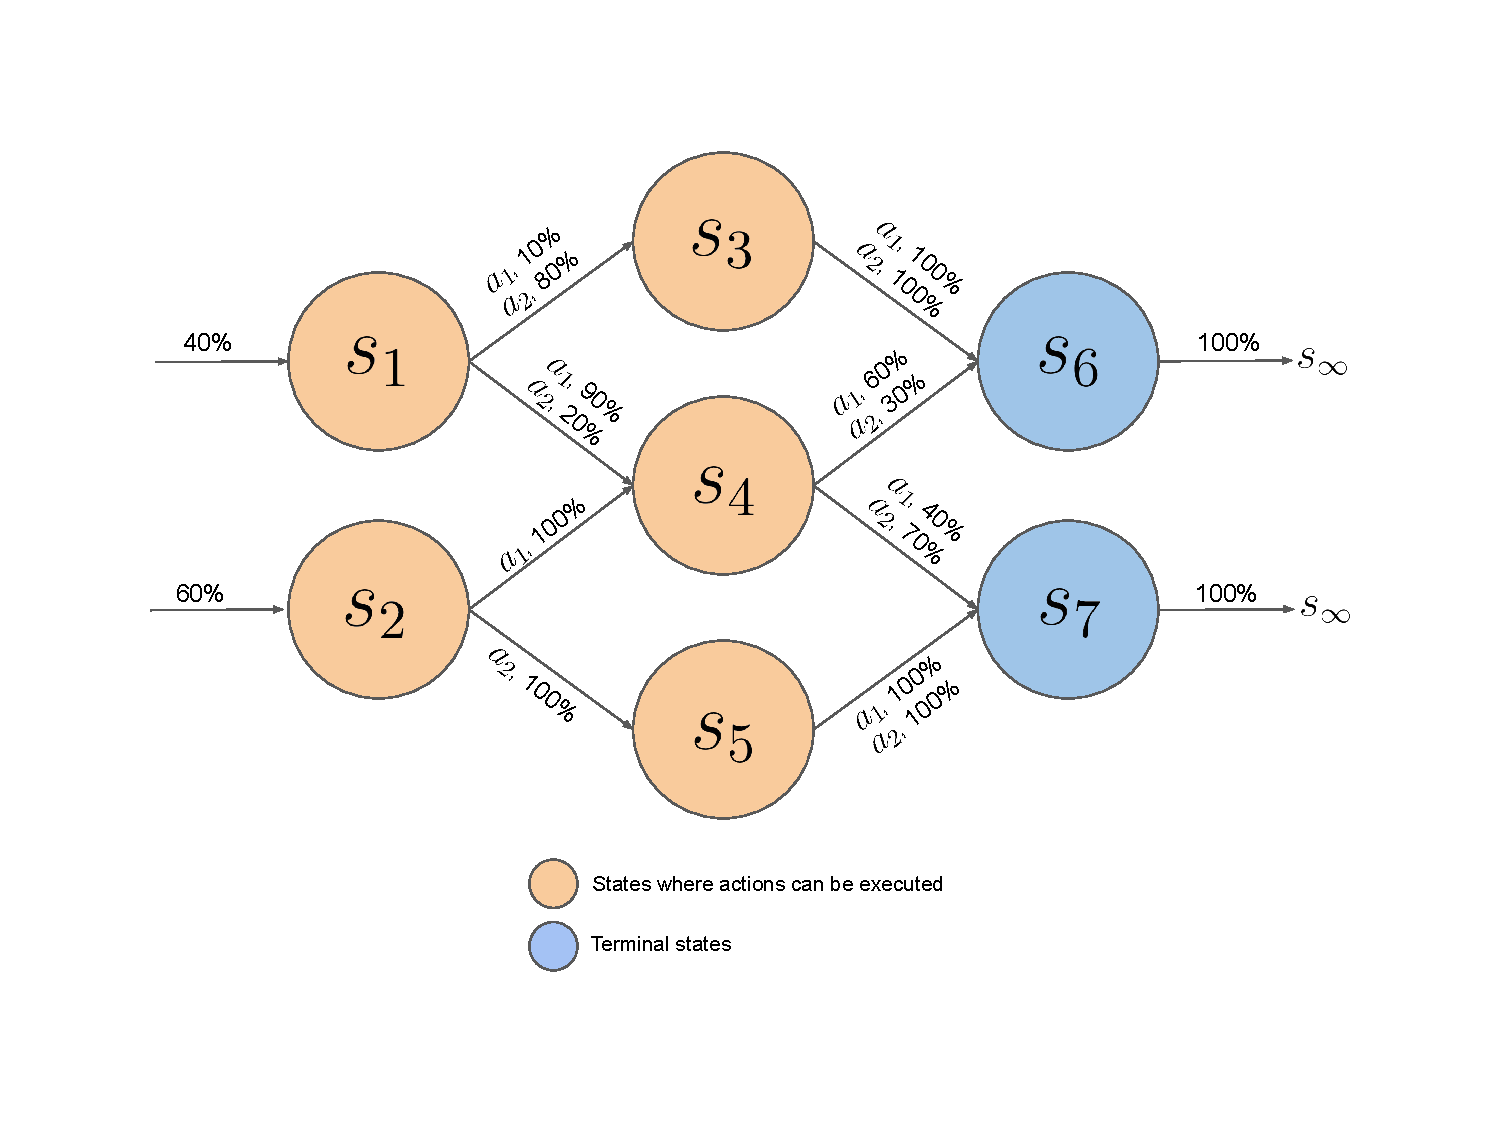
\includegraphics[width=0.8\textwidth]{HW_figs/HW1_MDP.pdf}
    \caption{An MDP.}
\end{figure}

\noindent Assume the following initial state distribution, $d_0$, and transition function, $p$, where all transition probabilities not indicated in the table below are $0$.

\begin{table}[h!!!]
\centering
\begin{tabular}{|l|l|}
\hline
$d_0(s_1)=0.4$ & $d_0(s_2)=0.6$ \\ \hline
$p(s_1,a_1,s_3)=0.1$    &   $p(s_1,a_1,s_4)=0.9$ \\ \hline
$p(s_1,a_2,s_3)=0.8$    &   $p(s_1,a_2,s_4)=0.2$ \\ \hline
$p(s_2,a_1,s_4)=1.0$    &   $p(s_2,a_2,s_5)=1.0$ \\ \hline
$p(s_3,a_1,s_6)=1.0$    &   $p(s_3,a_2,s_6)=1.0$ \\ \hline
$p(s_4,a_1,s_6)=0.6$    &   $p(s_4,a_1,s_7)=0.4$ \\ \hline
$p(s_4,a_2,s_6)=0.3$    &   $p(s_4,a_2,s_7)=0.7$ \\ \hline
$p(s_5,a_1,s_7)=1.0$    &   $p(s_5,a_2,s_7)=1.0$ \\ \hline
\end{tabular}
\end{table}

\noindent Assume the following reward function:

\begin{table}[h!!]
\centering
\begin{tabular}{|l|l|}
\hline
$R(s_1,a_1)=5$ & $R(s_1,a_2)=2$ \\ \hline
$R(s_2,a_1)=-3$ & $R(s_2,a_2)=7$ \\ \hline
$R(s_3,a_1)=3$ & $R(s_3,a_2)=-5$  \\ \hline
$R(s_4,a_1)=-6$ & $R(s_4,a_2)=8$ \\ \hline
$R(s_5,a_1)=4$ & $R(s_5,a_2)=10$ \\ \hline
\end{tabular}
\end{table}

\newpage

\noindent Finally, consider the following stochastic policy, $\pi$:

\begin{table}[h!!]
\centering
\begin{tabular}{|l|l|}
\hline
$\pi(s_1,a_1)=0.4$ & $\pi(s_1,a_2)=0.6$  \\ \hline
$\pi(s_2,a_1)=0.35$ & $\pi(s_2,a_2)=0.65$ \\ \hline
$\pi(s_3,a_1)=0.9$ & $\pi(s_3,a_2)=0.1$  \\ \hline
$\pi(s_4,a_1)=0.5$ & $\pi(s_4,a_2)=0.5$ \\ \hline
$\pi(s_5,a_1)=0.1$ & $\pi(s_5,a_2)=0.9$  \\ \hline
\end{tabular}
\end{table}


\vspace{0.5cm}
\noindent\rule{\textwidth}{1pt}
\vspace{0.1cm}


\noindent \textbf{(Question 1. \POINTS{15 Points})} Find an analytic, closed-form expression for
\begin{eqnarray*}
J(\pi) &=& \mathbb{E}\left[  \sum_{t=0}^1 \gamma^t R_t\right]
\end{eqnarray*}
as a function of $\gamma$. To do this, you \textit{may} choose do it from ``first principles'', by repeatedly using the properties of probability distributions and expected values introduced in Section \ref{sec:hints}. If you do not wish to derive a closed-form expression for $J(\pi)$ this way, you are also allowed to write it directly as a function of $d_0$, $p$, $\pi$, and $R$, similarly to the final equation described in the ``\textbf{Example problem}'' introduced in Section \ref{sec:hints}.

Your final answer should be in the form of $J(\pi) = c_1 + \gamma c_2$, where each $c_i$ is a real-valued constant. Hint: start by applying the property of linearity of expectation to the definition of $J(\pi)$ and then derive separate equations for each of the resulting terms.
\\ \\
    %
    % YOUR RESPONSE HERE
    %
\textbf{(Question 2 - 30 Points)} \underline{\textbf{\textit{Programming Question}}}

\vspace{0.3cm}

In this question, you will write a program to estimate $J(\pi)$ by simulating many of the possible outcomes (returns) that might result from running $\pi$ on the previously-defined MDP. Each simulation will produce a particular sequence of states, actions, and rewards, and, thus, a particular discounted return. Since $J(\pi)$ is defined as the \textit{expected} discounted return, you can construct an estimate of $J(\pi)$, $\hat{J}(\pi)$, by averaging the discounted returns observed across $N$ simulations.
\\ \\ 
In particular:

\begin{itemize}
    \item To run one simulation (or episode, or trial), you should follow the ``Agent-Environment Interaction'' procedure introduced in Class \#3. 
    \item Start by creating a function called \textit{runEpisode} that takes as input a policy and a value of $\gamma$, and that returns the empirical discounted return resulting from that episode.
    \item Let $G^i$ be the discounted return of the $i^{th}$ episode. You will estimate $J(\pi)$ by computing $\hat{J}(\pi) := \frac{1}{N} \sum_{i=1}^N G^i$.
\end{itemize}
    %
    %
\textbf{(Question 2a. \POINTS{8 Points)}}. Construct $\hat{J}(\pi)$ by running 150,000 simulations/episodes. You should then create a graph where the $x$ axis shows the number of episodes, and the $y$ axis presents the estimate $\hat{J}(\pi)$ constructed based on all episodes executed up to that point. That is, the point $x=100$ in this graph should have as its corresponding $y$ coordinate the estimate $\hat{J}(\pi)$ built using the discount returns from the first $100$ simulations. \textcolor{blue}{\textbf{You should use $\gamma=0.9$. Using a value $\gamma < 1$ will make it easier for you to debug whether your implementation of $\hat{J}(\pi)$ matches the expected results given by the analytic solution you constructed in part 1 of this question. In case you have already solved this question using a different value of $\gamma$, that is ok: you can still submit your results as they are, but please \underline{\textbf{do report}} which value of $\gamma$ you chose to use.}}
\\ \\
    %
    % YOUR RESPONSE HERE
    %
\textbf{(Question 2b. \POINTS{5 Points)}}. Report the average discounted return, as well as its variance, at the end of this process; that is, report  $\hat{J}(\pi)$ after executing 150,000 episodes.
\\ \\
    %
    % YOUR RESPONSE HERE
    %
\textbf{(Question 2c. \POINTS{5 Points)}}. Estimate $\hat{J}(\pi)$ using different discount rates: $\gamma \in \{0.25, 0.5, 0.75, 0.99\}$. Compare these estimates with their true values, computed according to the closed-form solution for $J(\pi)$ found in the first part of this question. These values should approximately match (i.e., $J(\pi) \approx \hat{J}(\pi)$).
\\ \\
    %
    % YOUR RESPONSE HERE
    %
\textbf{(Question 2d. \POINTS{12 Points)}}. Next, we will use your \textit{runEpisode} function to estimate the performance of \textit{different} policies (other than the one we introduced/proposed) in order to search for the policy with highest performance. You may use any optimization method you want to implement this step (even, e.g., brute force search). To simplify this process, you \textit{should} restrict your search to deterministic policies. You should use $\gamma=0.75$. Describe how the policy search method you used works. Report the best policy, $\hat{\pi}^*$, identified by the process above, and present its estimated performance, $\hat{J}(\hat{\pi}^*)$, computed using $N=350,000$ simulations.
    %
    % YOUR RESPONSE HERE
    %
\end{document}
